\setlength{\parskip}{\baselineskip} 
%\section{\bnmf}

\frame{\frametitle{Simulations}
%\begin{overlayarea}{\textwidth}{\textheight}
\begin{columns}
\column{0.5\textwidth}
%\vspace{1}
\begin{itemize}
	\item Matrix size
	\begin{itemize}
		\item 1,000 $\times$ 40
		\end{itemize}
	\item Low rank structure
	\begin{itemize}
		\item Rank: 4
		\end{itemize}
	\item Increasing noise
	\begin{itemize}
		\item Low $\longrightarrow$ High
		\end{itemize}
	\item Compared with 
		\begin{itemize}
		\item PCA
		\item Factor analysis
		\item NMF
			\end{itemize}
\end{itemize}
\column{0.5\textwidth}
\vspace{1em}
\begin{center}
\only<1>{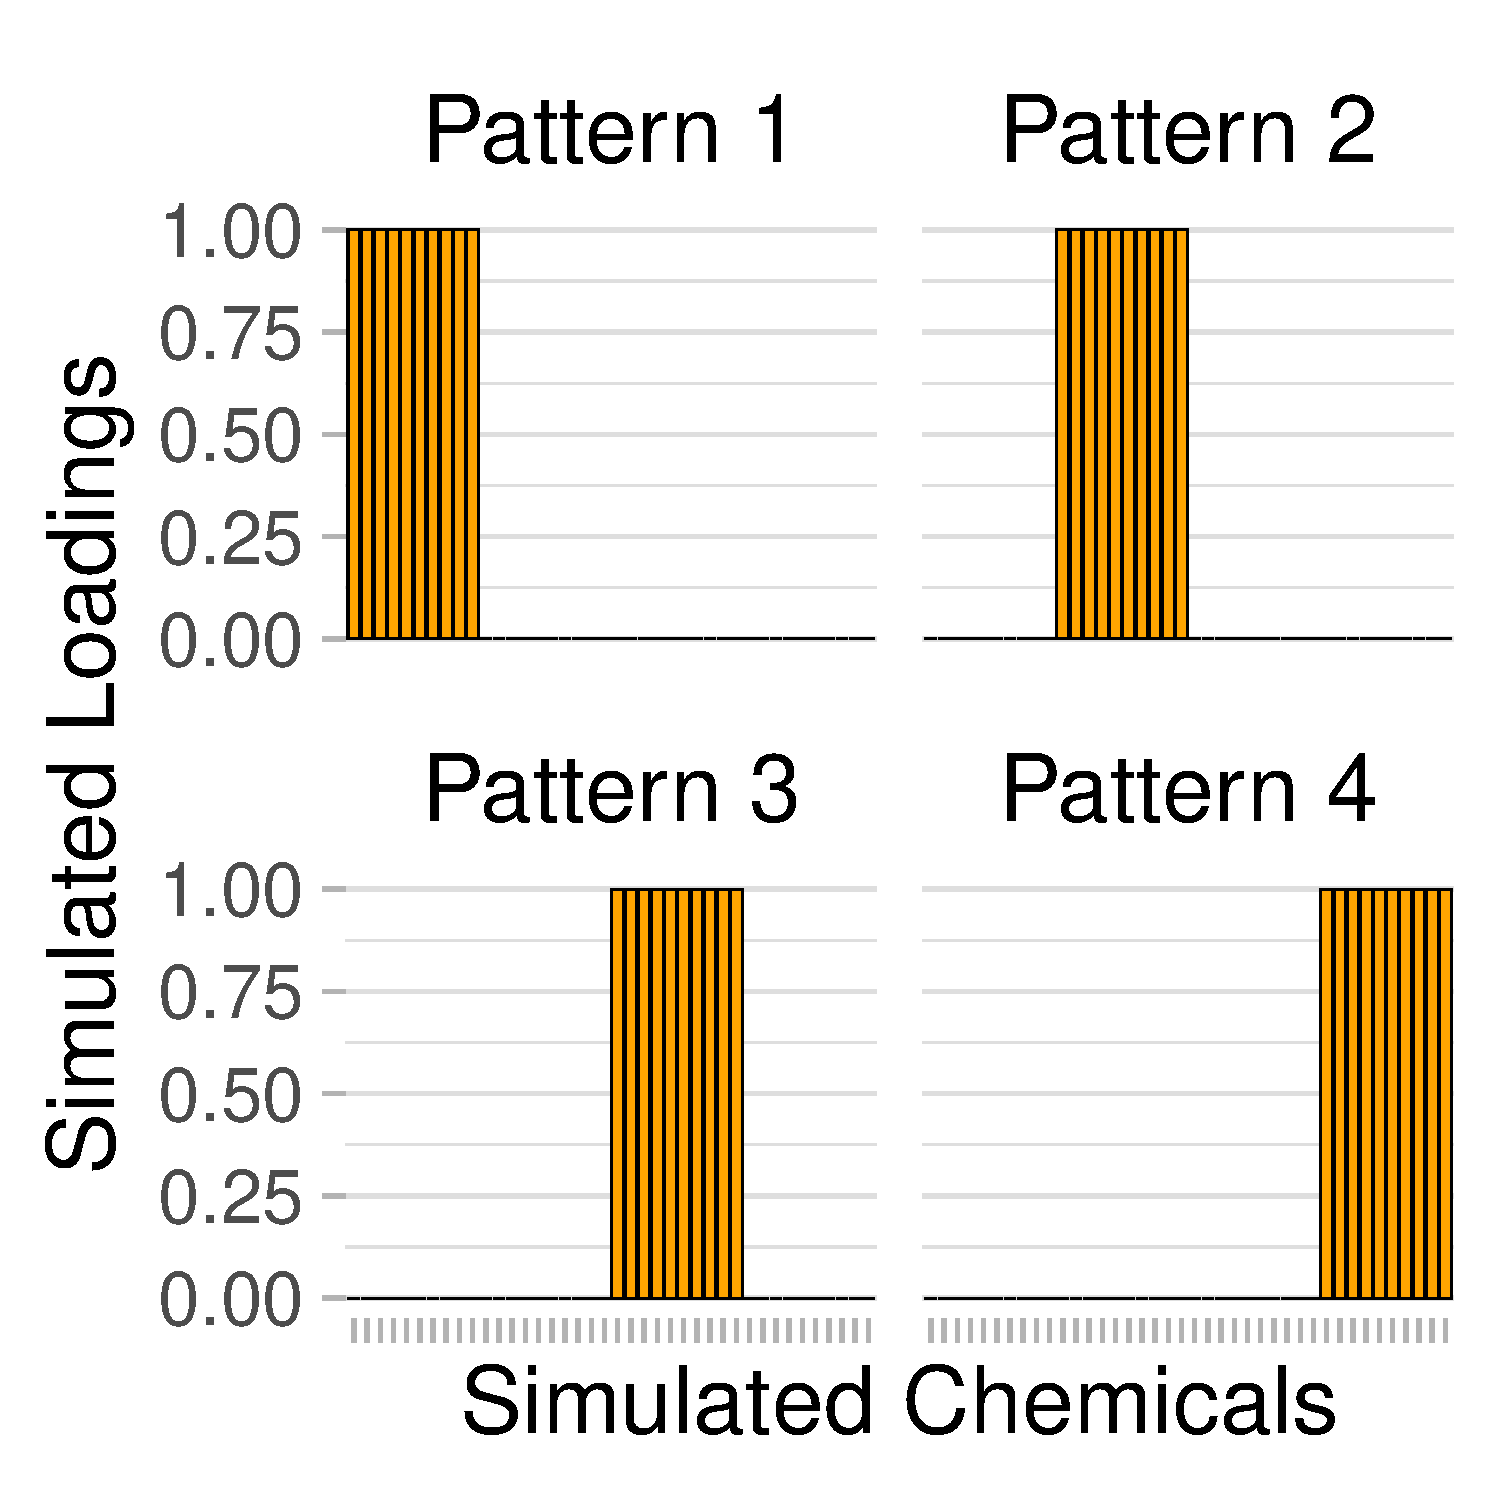
\includegraphics[height=5cm]{figures/bn2mf/loadings_plot0.pdf}}
\only<2>{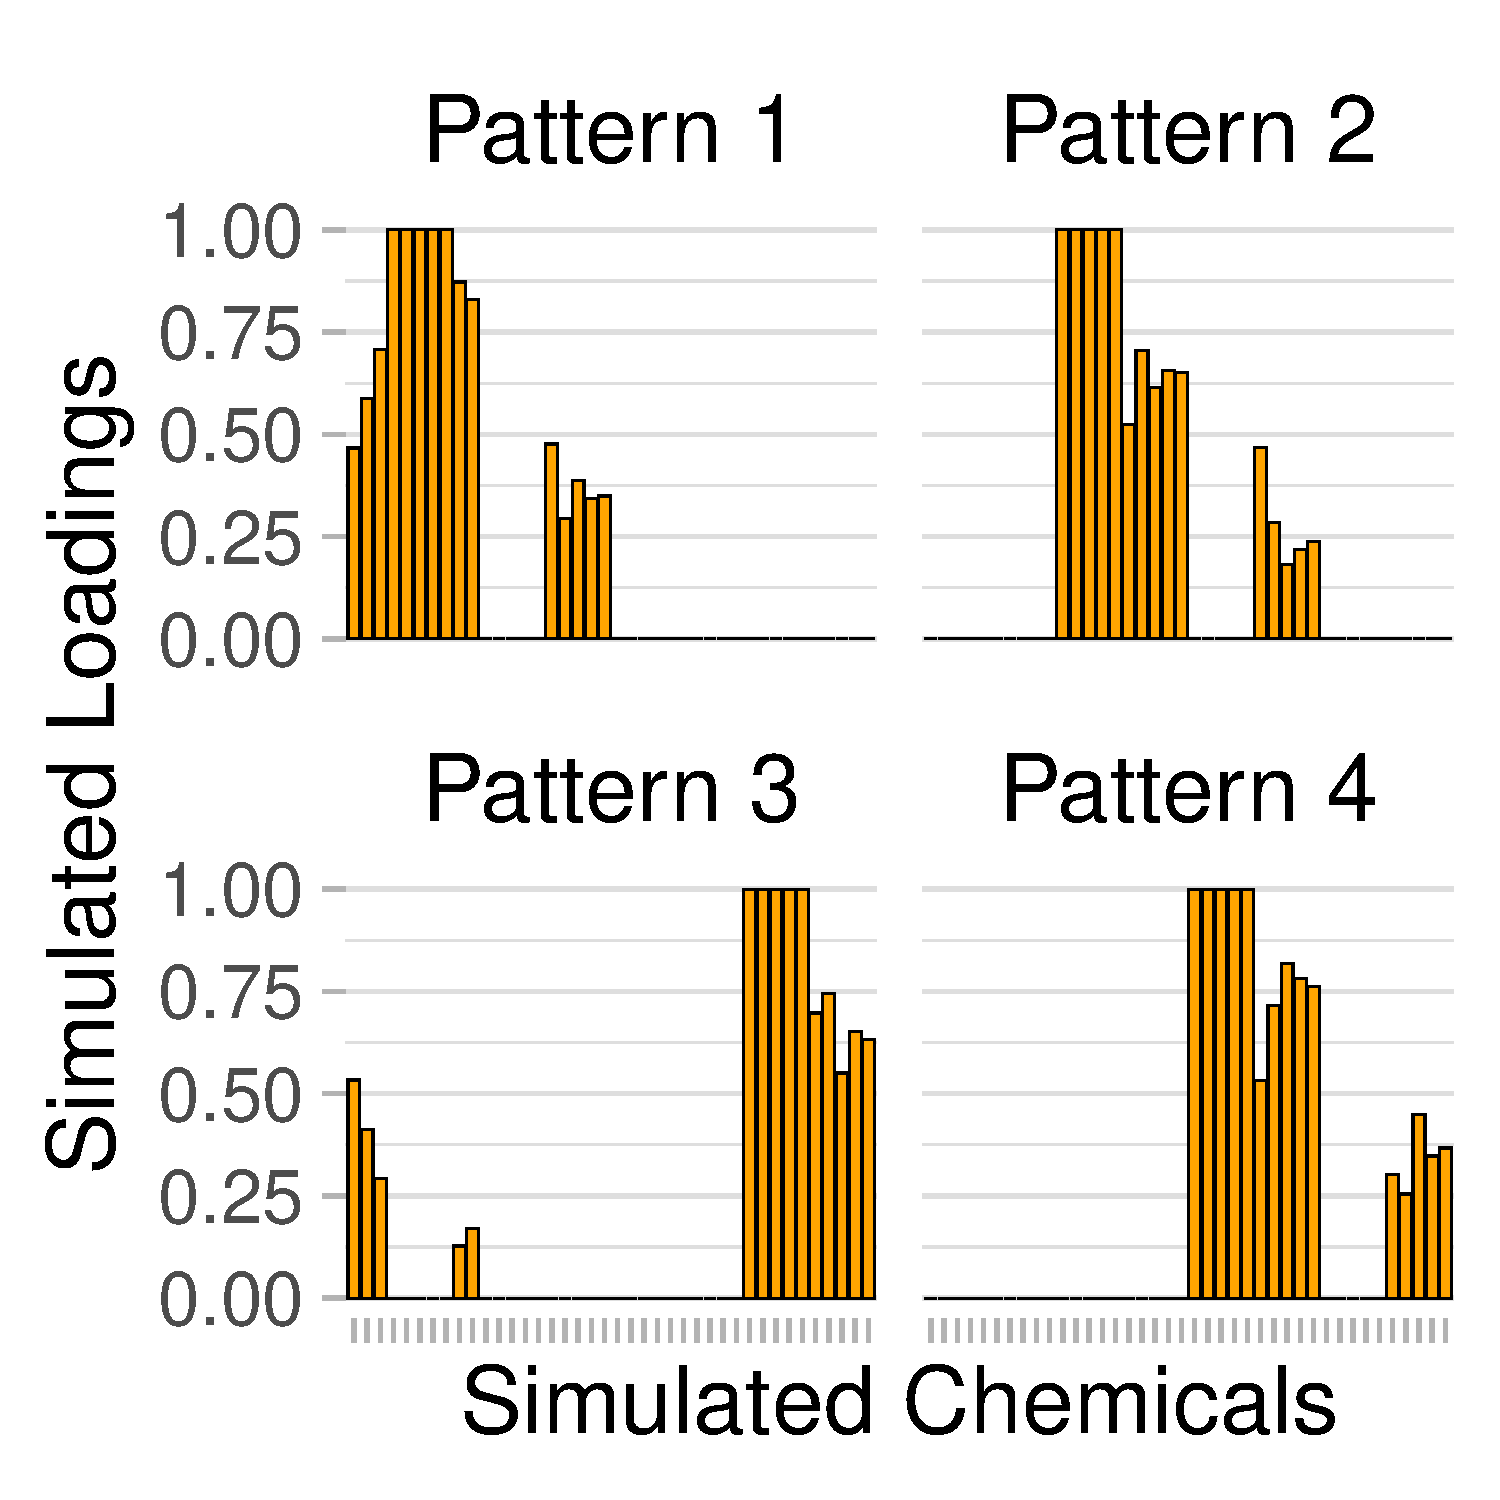
\includegraphics[height=5cm]{figures/bn2mf/loadings_plot5.pdf}}
\only<3>{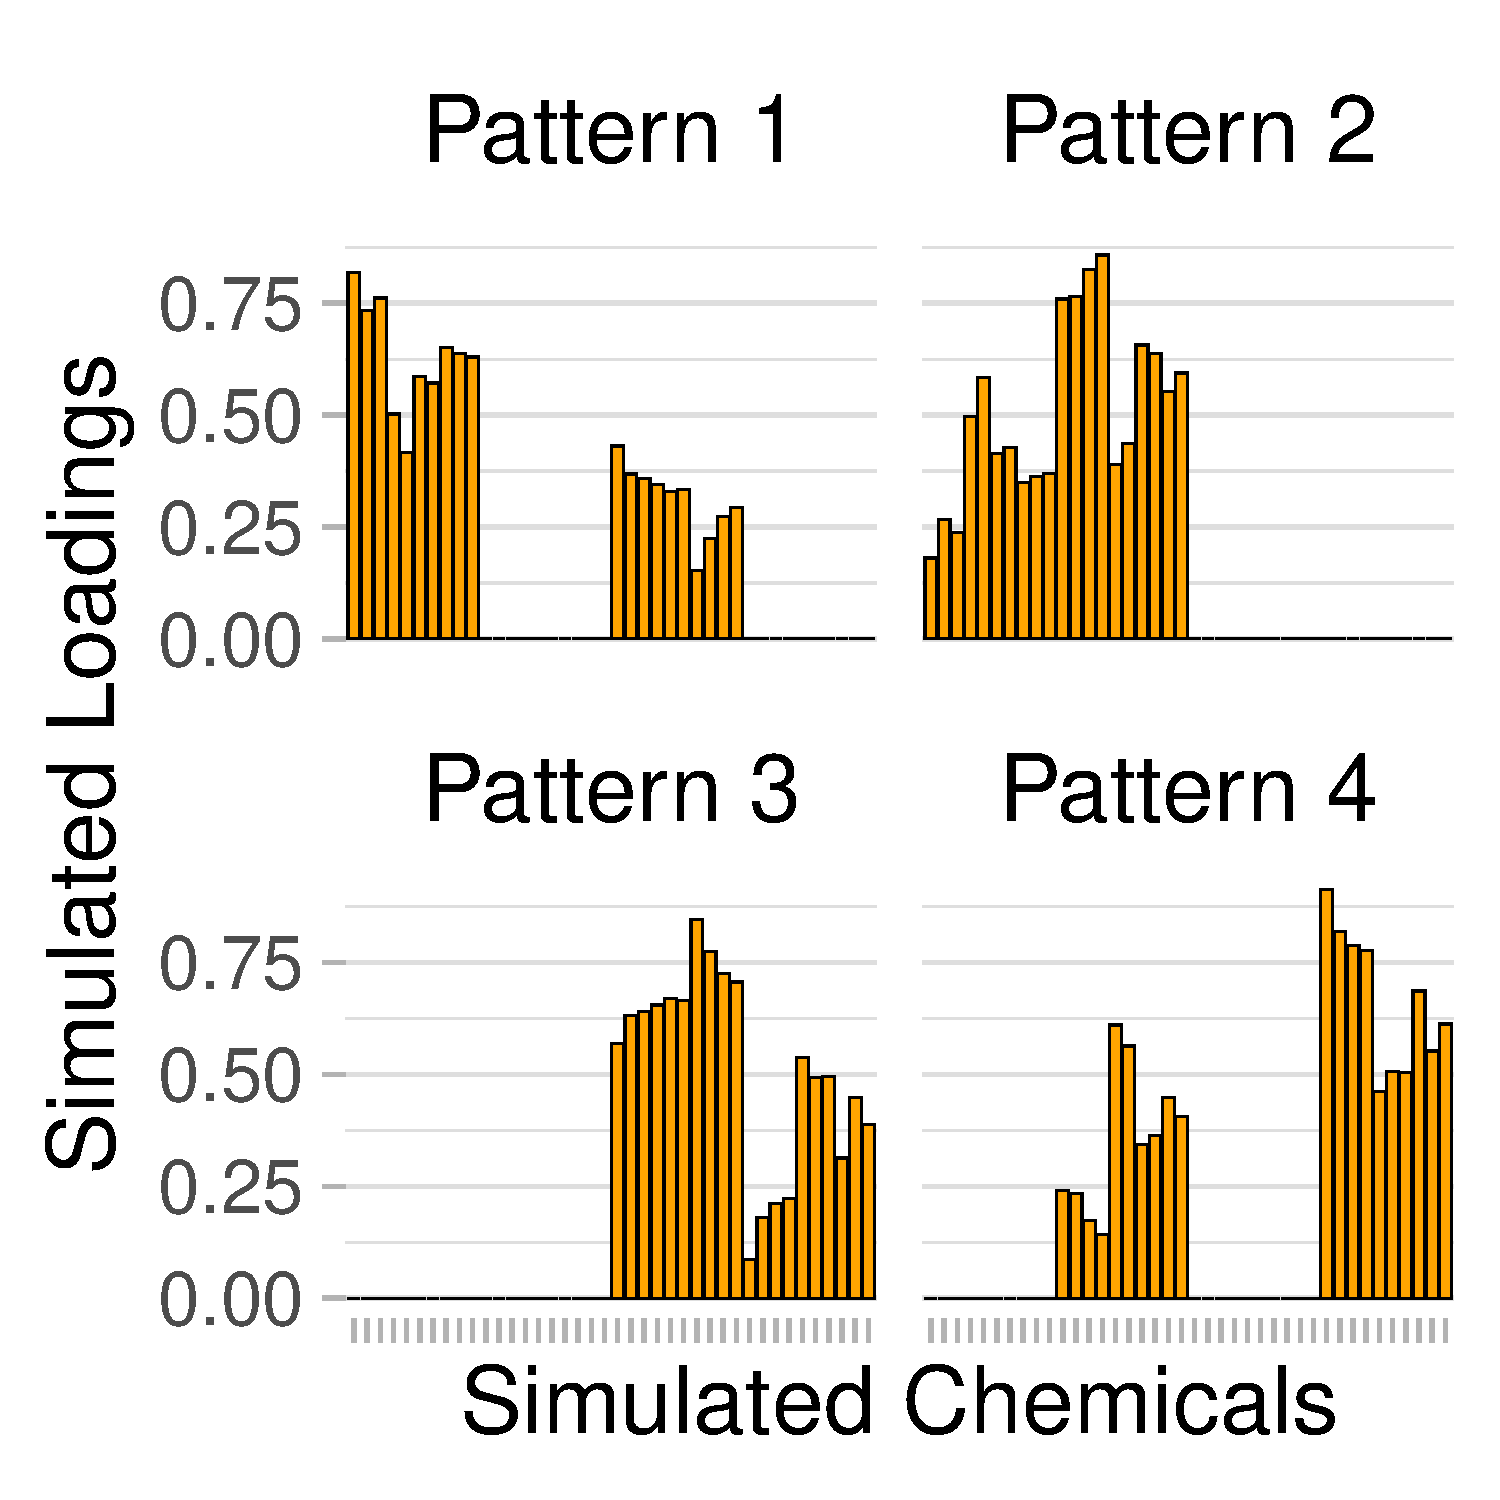
\includegraphics[height=5cm]{figures/bn2mf/loadings_plot10.pdf}}
\only<4>{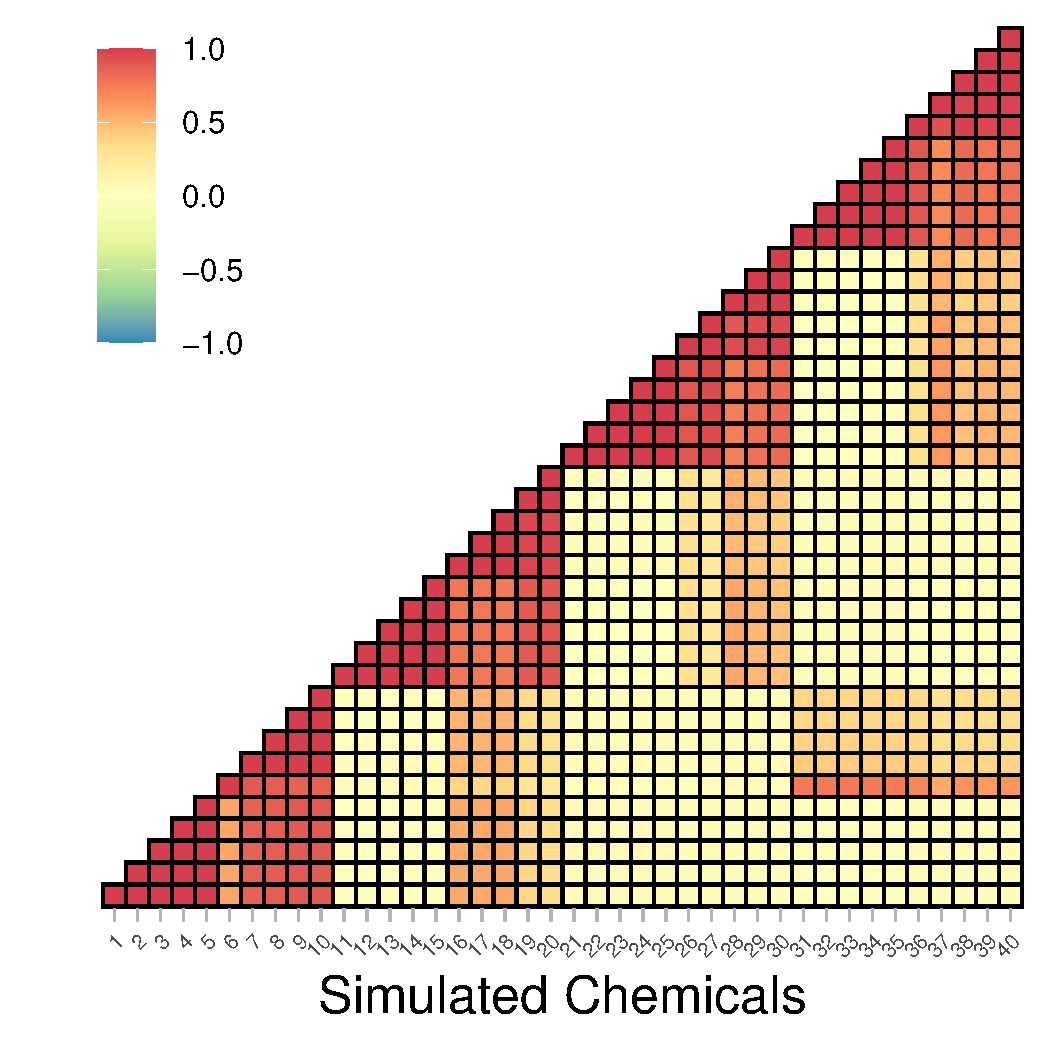
\includegraphics[height=5cm]{figures/bn2mf/sim_corr_bn2mf.pdf}}
\end{center}
\end{columns}
%\end{overlayarea}
}

% \frame{\frametitle{Simulations}
% \vspace{2ex}
% \begin{columns}
% \column{0.5\textwidth}

% \column{0.5\textwidth}

% \begin{center}
%       \only<1>{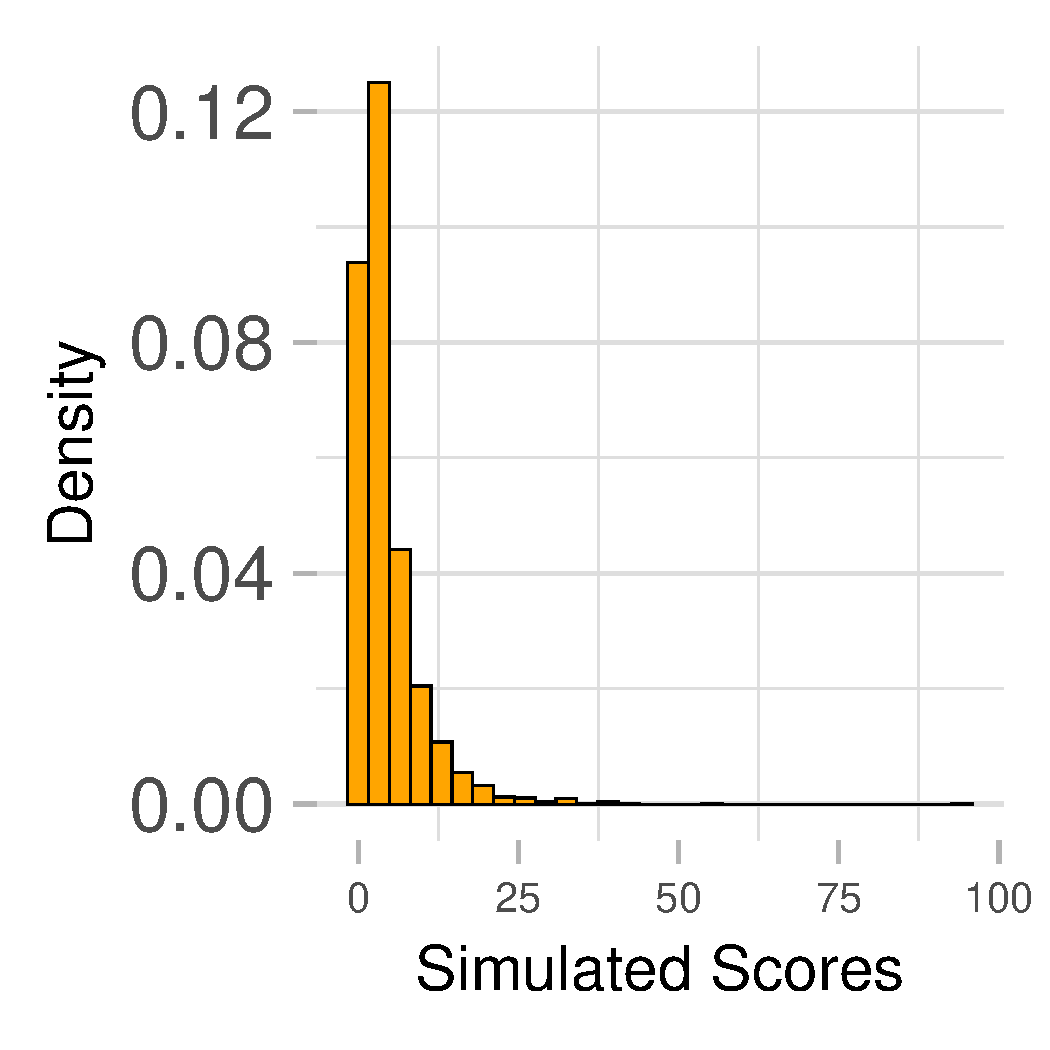
\includegraphics[scale = 0.3]{figures/pcp/scores_plot.pdf}}      \only<2>{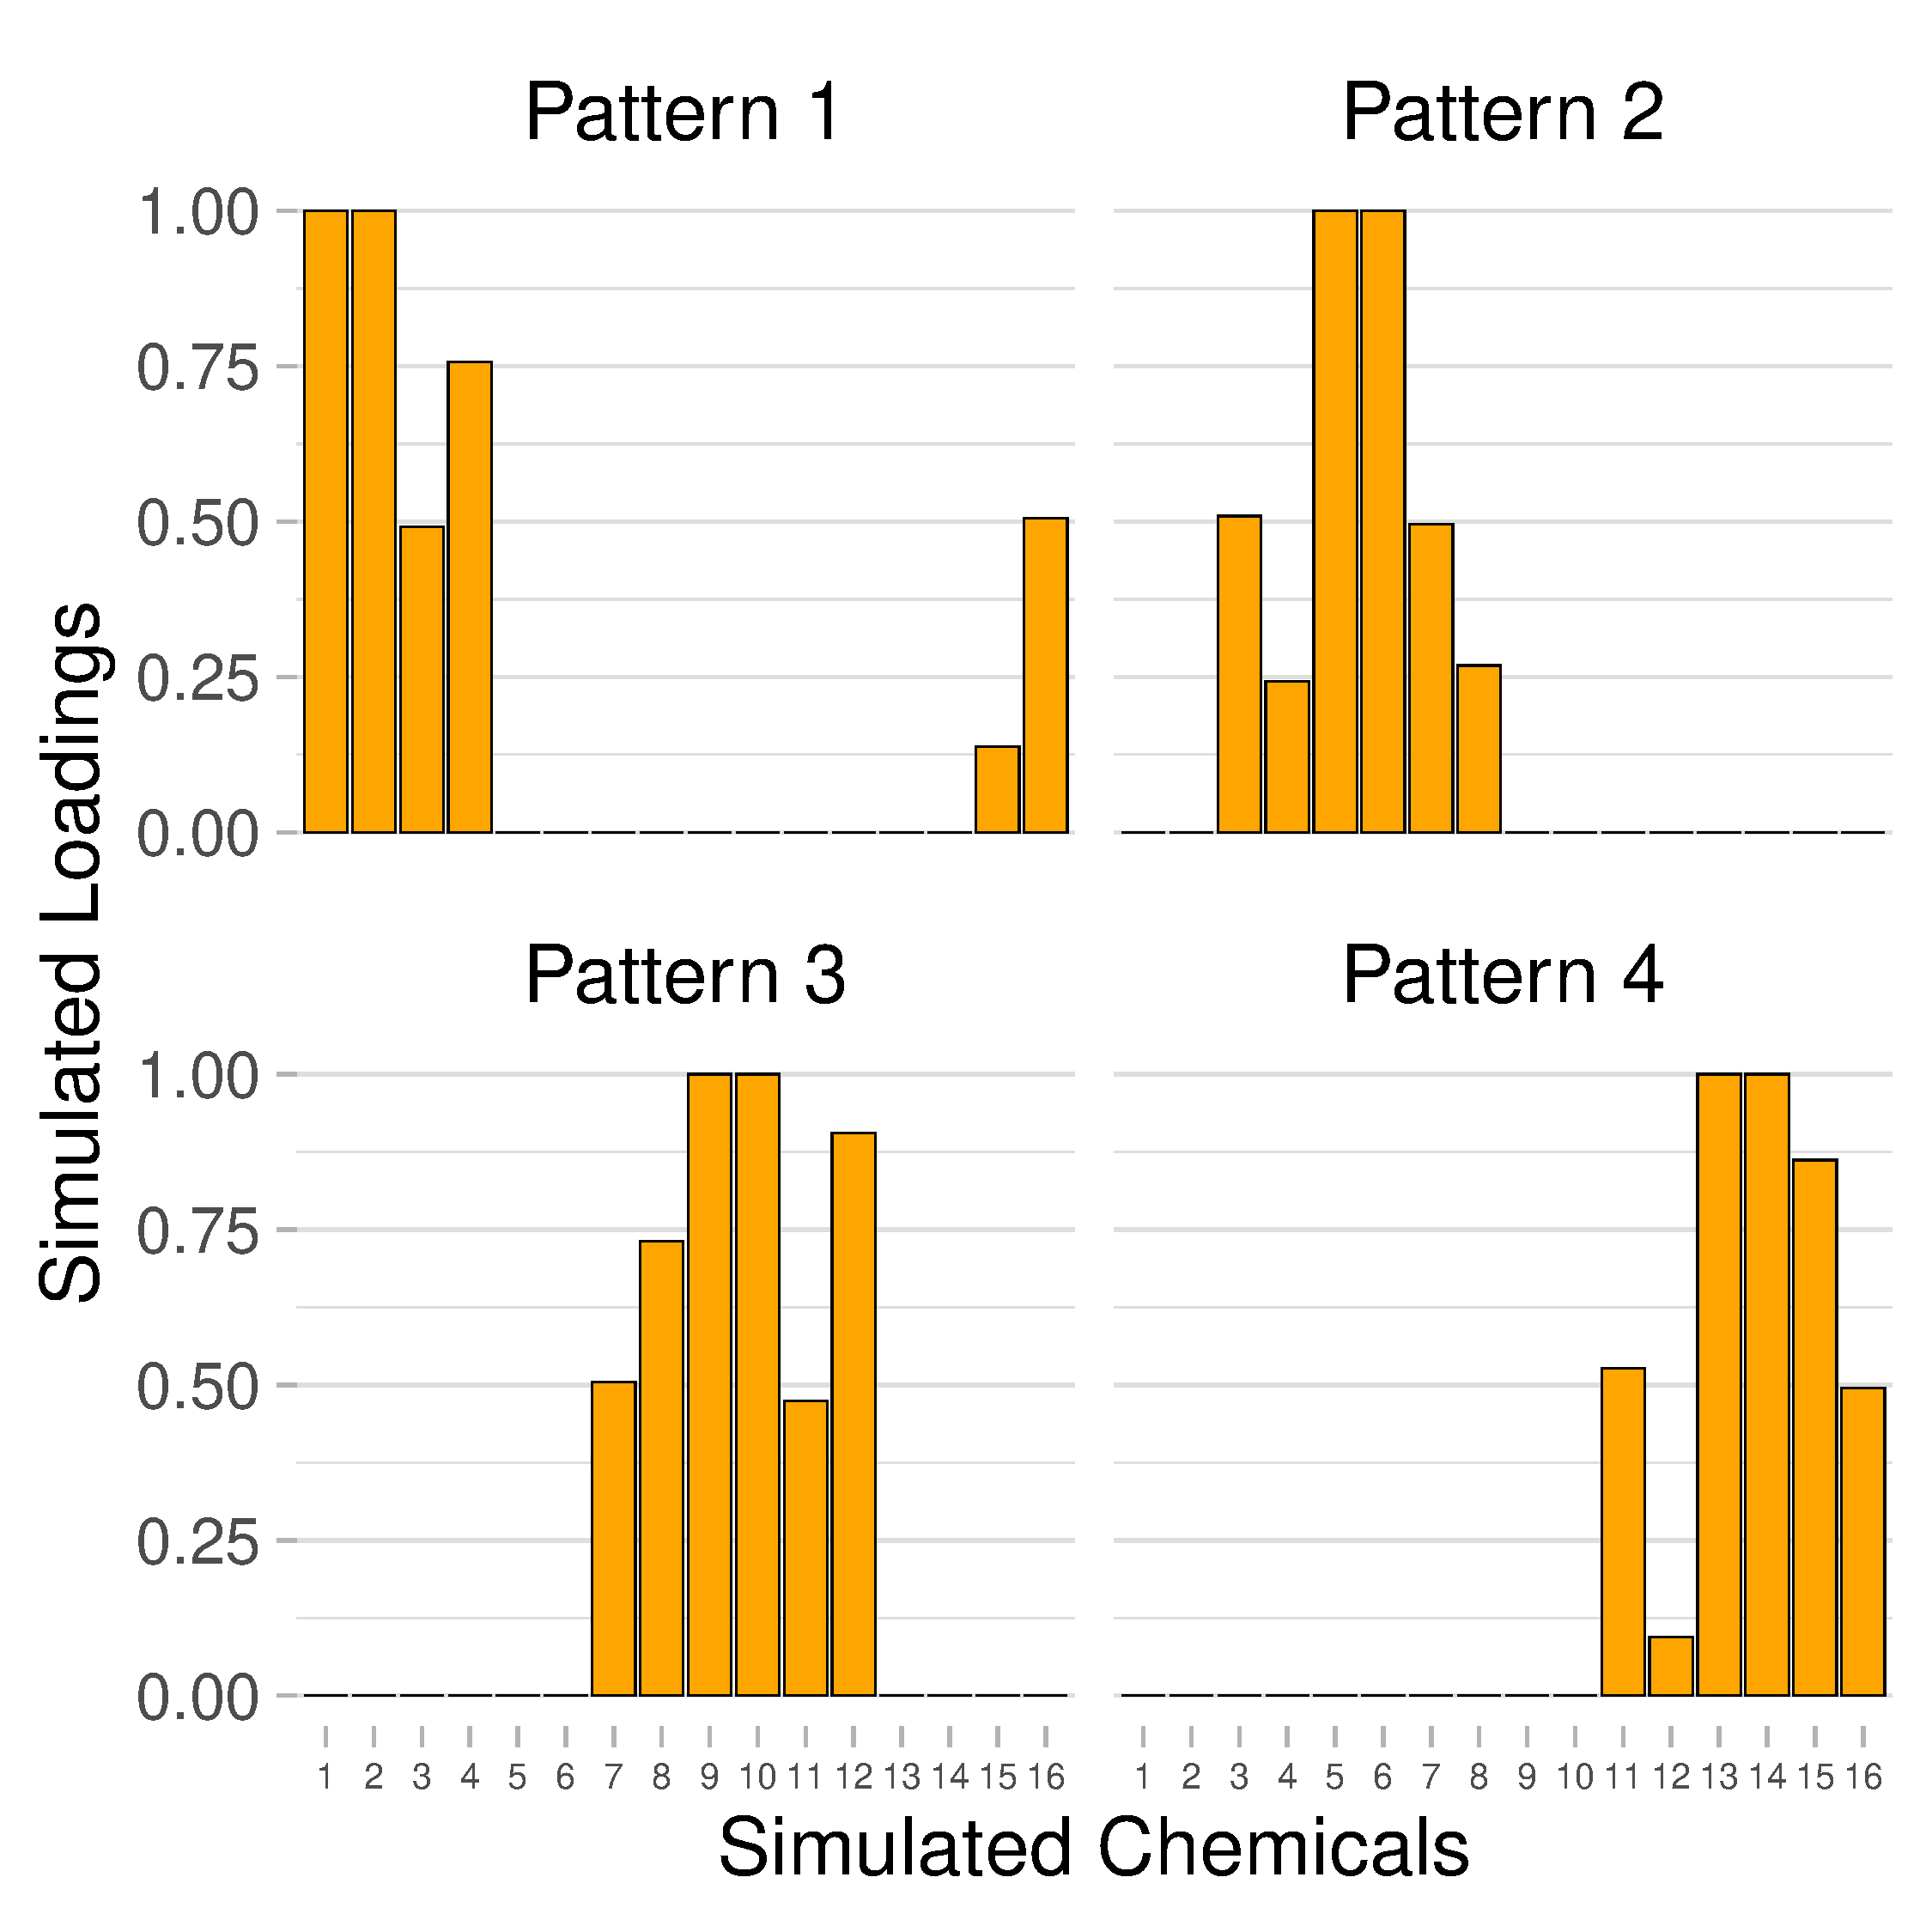
\includegraphics[scale = 0.14]{figures/pcp/loadings_plot.pdf}}
%       \only<3>{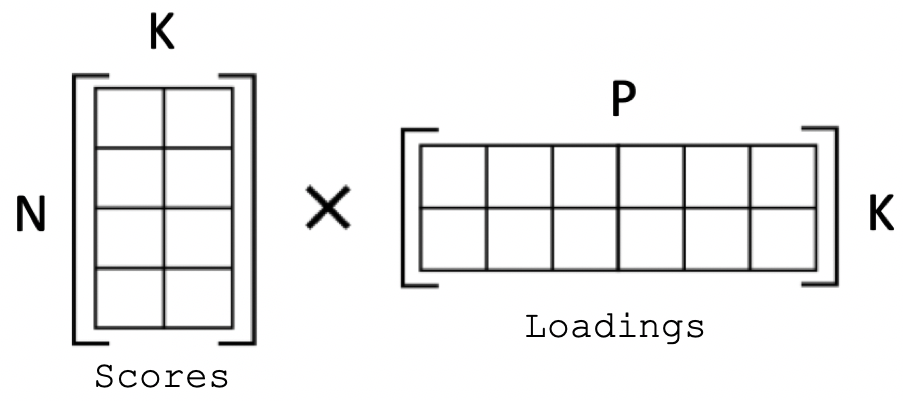
\includegraphics[scale = 0.35]{figures/patscore.png}}
%       \only<4>{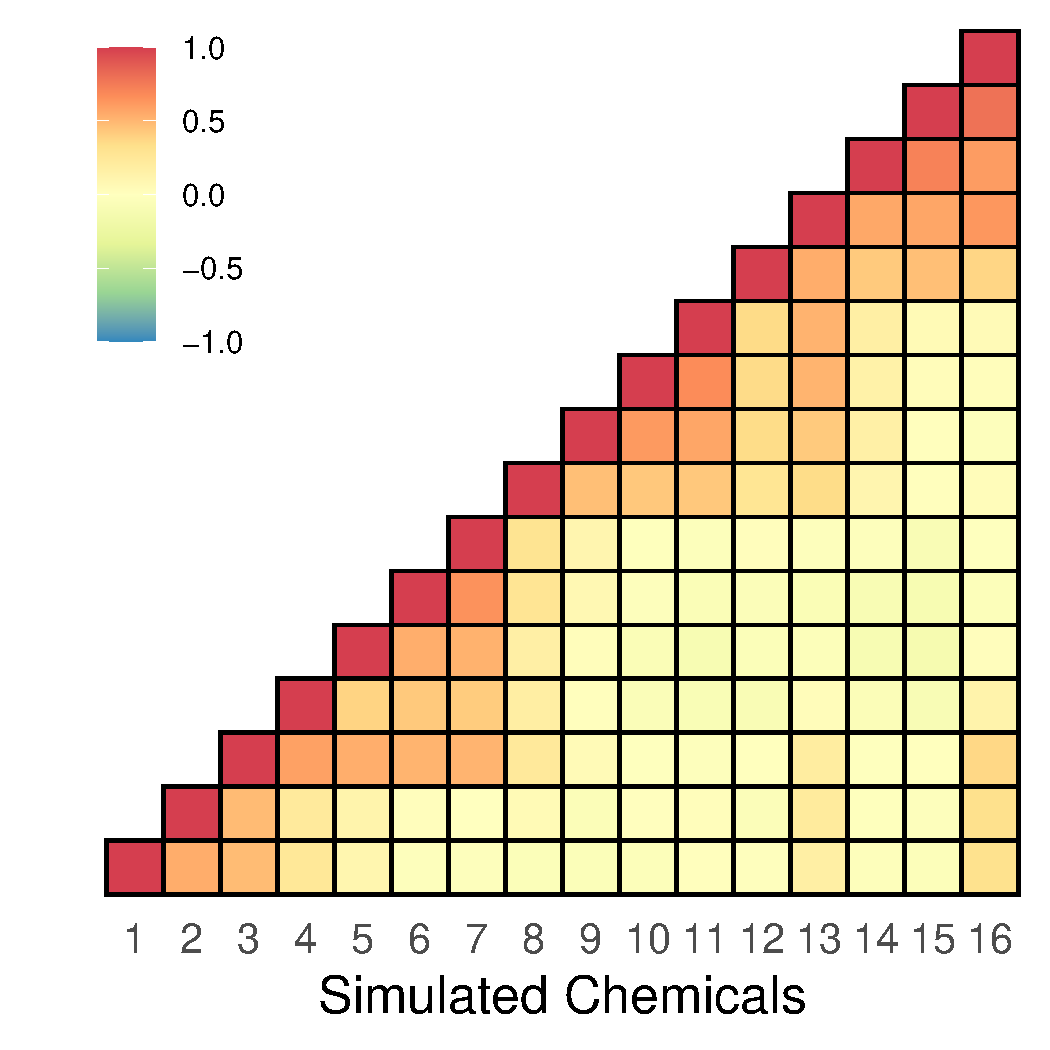
\includegraphics[scale = 0.3]{figures/pcp/sim_corr.pdf}}
% \end{center}
% \end{columns}
% }

\frame{
\frametitle{Relative overall error}
\vspace{-1ex}
\centering{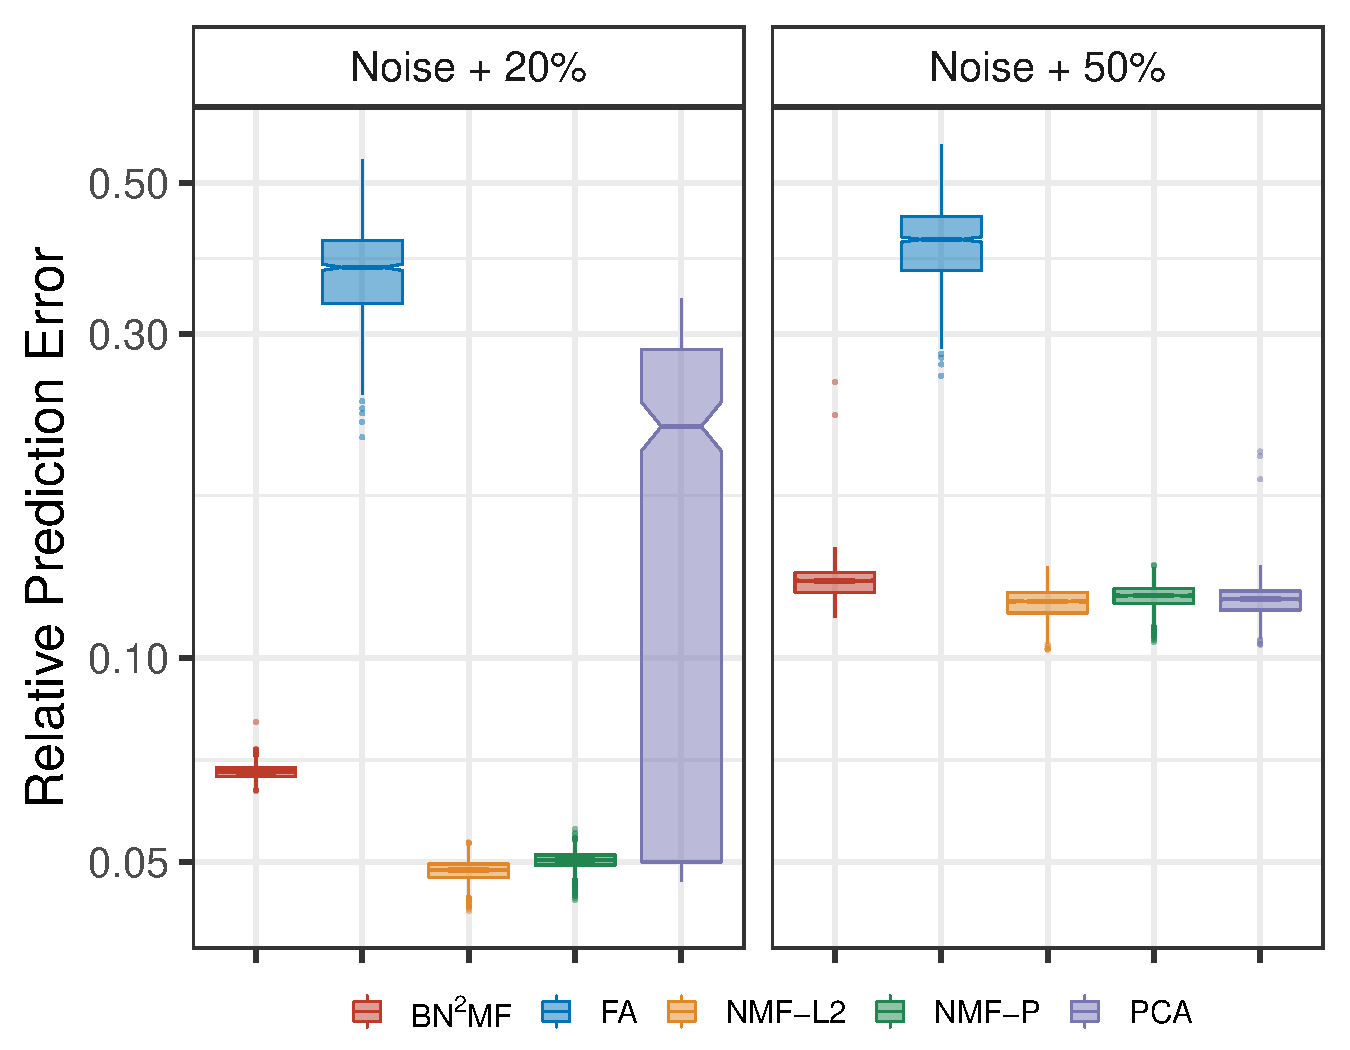
\includegraphics[scale = 0.4]{figures/bn2mf/prez_error.pdf}}
}

\frame{
\frametitle{95\% variational confidence interval coverage}
\centering{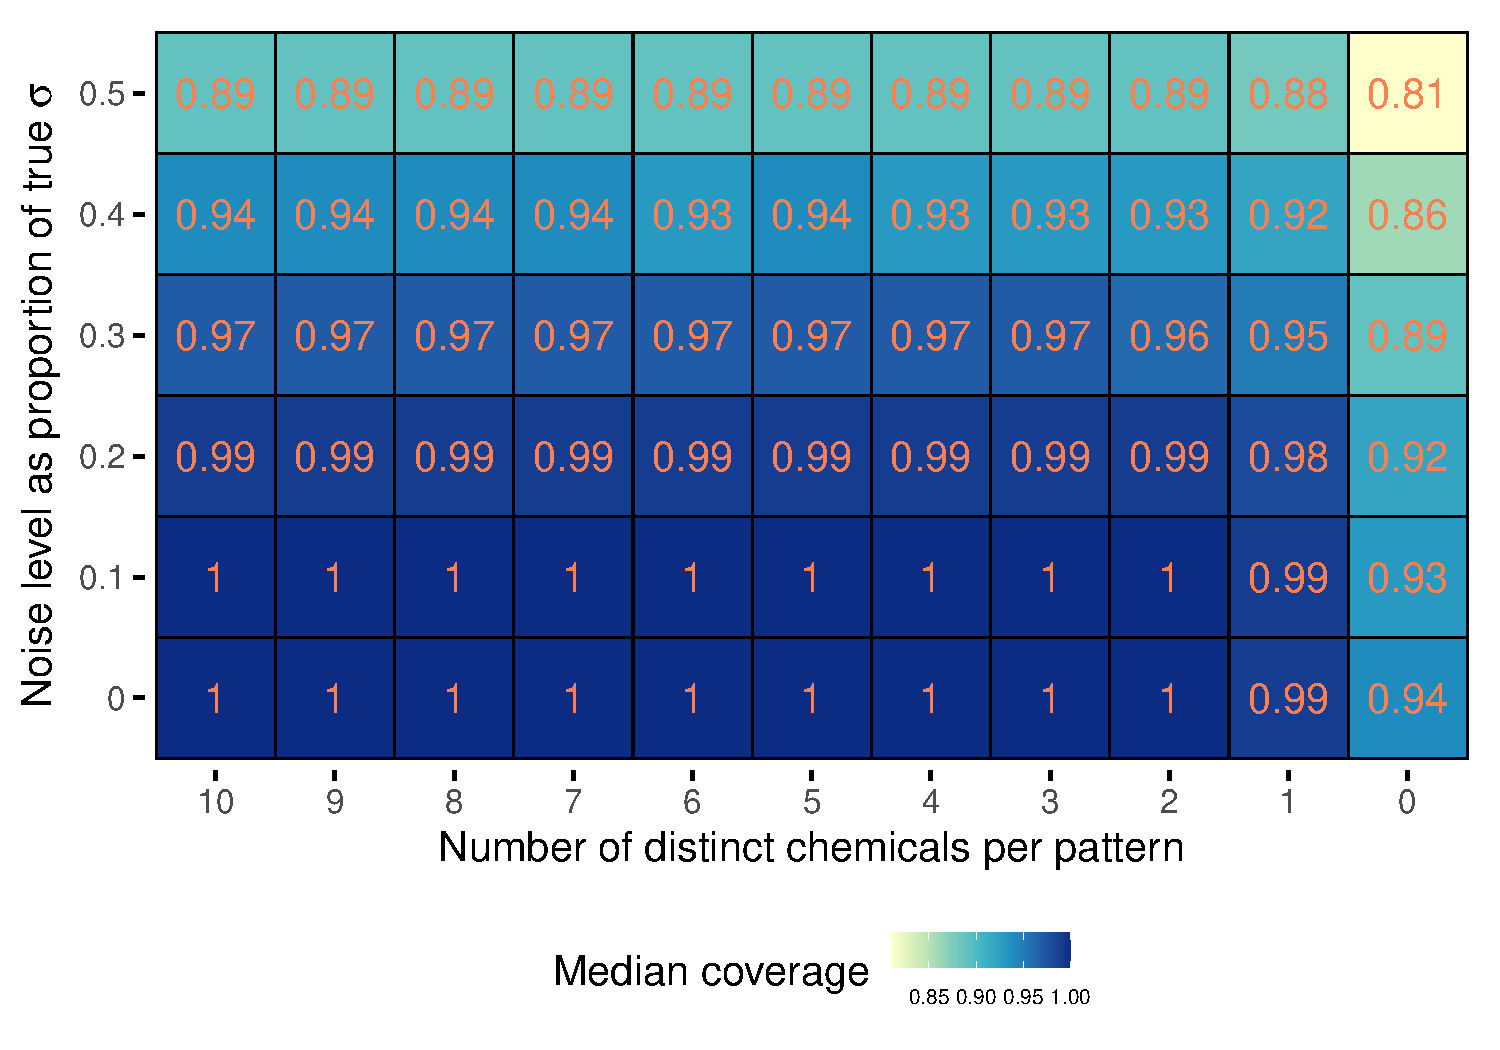
\includegraphics[scale = 0.4]{figures/bn2mf/coverage_heat_crop.pdf}}
}

\frame{
\frametitle{What do variational confidence intervals tell us?}
\centering{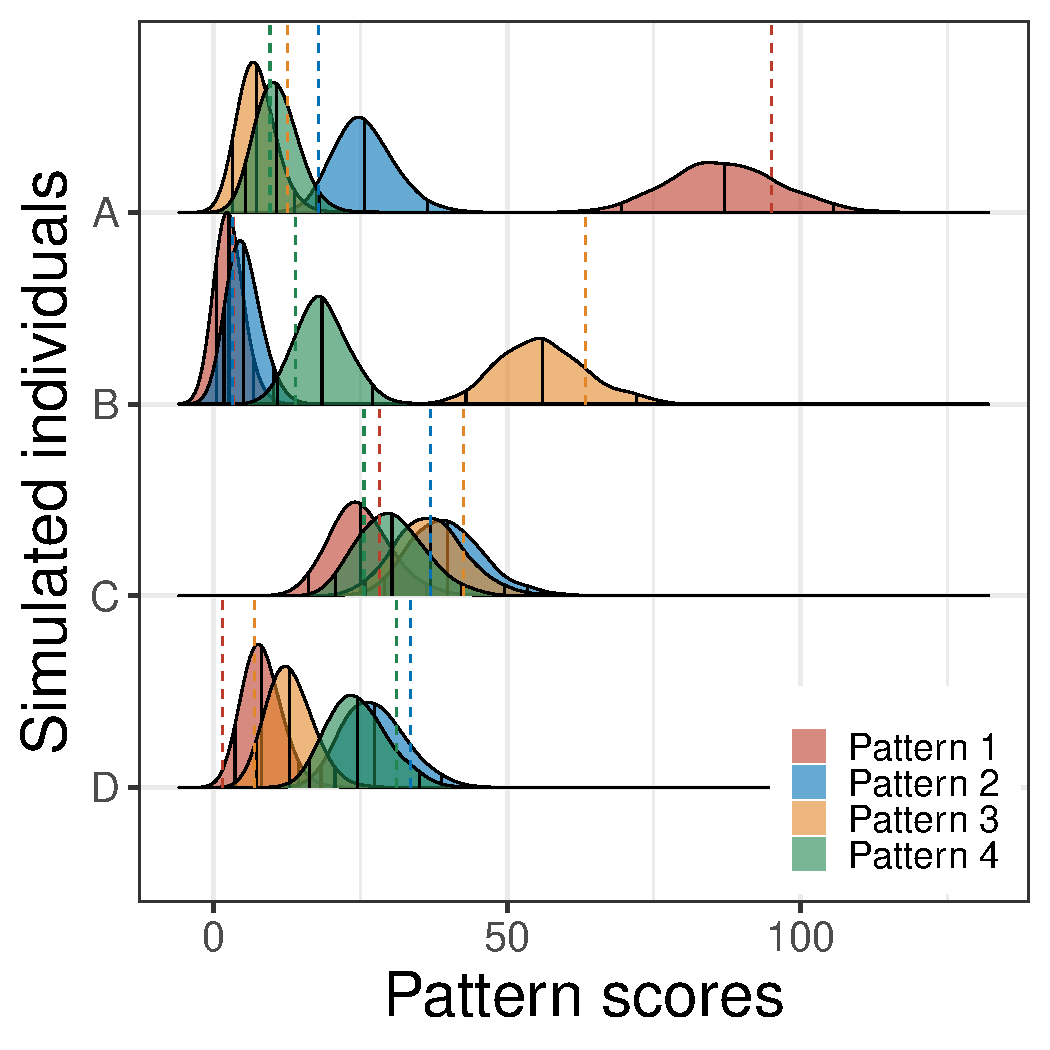
\includegraphics[scale = 0.41]{figures/bn2mf/ridges.pdf}}
\pause
\begin{tikzpicture}[overlay,remember picture]
        \pgftransformshift{\pgfpointanchor{current page}{center}}
        \node[rounded corners,
            draw=matbluedark,
            ultra thick,
            fill=white,
            %font=\LARGE,
            text width=0.3\textwidth,
            align=center,
            anchor=center
            ] at (3.5cm,1.45ex) {VCI give a range of possible values instead of a point estimate.
            };
    \end{tikzpicture}
}